\documentclass[main]{subfiles}
\begin{document}
\section{Transconductance Amplifier}
%Roland
\begin{figure}[b]
\begin{subfigure} [b]{0.45\textwidth}
  \centering
  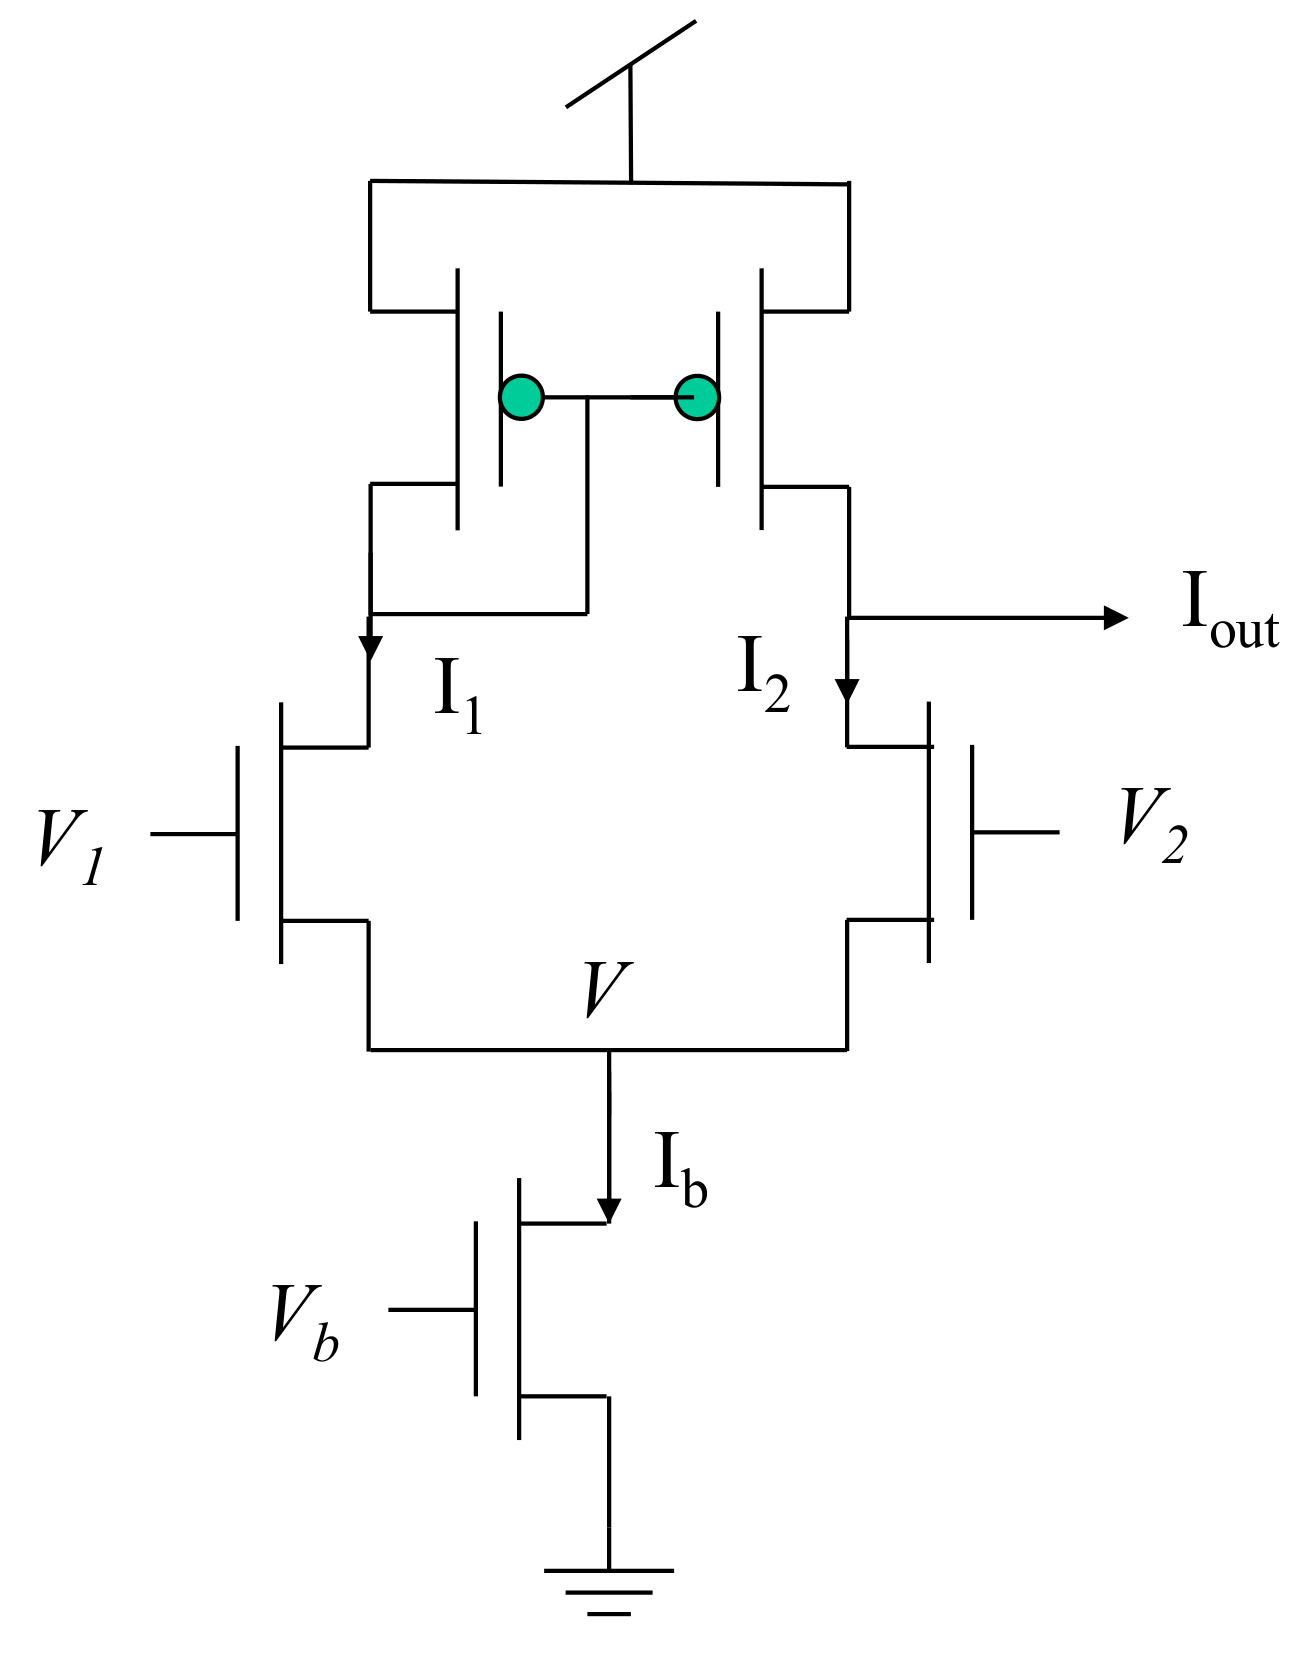
\includegraphics[scale=0.5]{pics/transamp.png}
  \caption{Circuit layout. \cite{lec4}}
  \label{fig:transamp}
\end{subfigure}
	\begin{subfigure} [b]{0.45\textwidth}
	\centering
	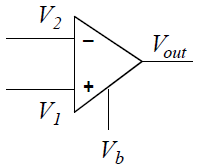
\includegraphics[scale=1]{pics/transcondamp_sym.png}
	\caption{Circuit symbol. \cite{lec5}}
	\label{fig:transamp_sym}
	\end{subfigure}
	\label{fig:transamp_all}
	\caption{A simple transconductance amplifier.}
\end{figure}\bigskip

The simple transconductance amplifier is very easy to understand if you know how the differential pair and the current mirror works, so check back if you don't. 

The bottom part of the transconductance amplifier (Fig. \ref{fig:transamp}) is a differential pair with a current mirror from one of the two outputs to the other one. What now happens is that the current $I_1$ get mirrored on top of $I_2$. We assume that $V_1$ and $V_2$ are not equal, and so aren't $I_1$ and $I_2$. The difference between the two currents then flows in or out of the amplifier in a way that Kirchhoff's current law is fulfilled:
$$I_{out} = I_1 - I_2 = I_b \tanh\left(\kappa \frac{V_1-V_2}{2U_T}\right)$$
Or for a small differential input ($|V_1-V_2| < 200 mV$):
$$ I_{out} \approx g_m \left(V_1-V_2\right) \text{  with  } g_m \approx \frac{\kappa I_b}{2U_T}$$
Since amplifiers are usually used in voltage and not in current mode, we focus on its behavior when the output current $I_{out}$ is fixed. Let's set $V_1 = V_2$ such that $I_{out}$ is zero and keep it there. If we now increase for example $V_2$, the corresponding transistor would drain more current, which can't be provided by the upper transistor since it only mirrors $I_1$. In order to fulfill all transistor equations and Kirchhoff's current law, $V_{out}$ decreases such that the lower transistor is no longer in saturation. Since the transistors behave exponential, even a small change of the input voltages leads to a big change in the output voltage.
\par For this amplifying behavior, it is very important that all transistors operate in saturation region. We already know the common node voltage is 
$ V = \kappa \left(\max \left(V_1, V_2\right)-V_b \right)$ if $|V_1 - V_2| > 4U_T$. Therefore, the saturation condition for the bias transistor is
$\max \left(V_1, V_2\right) > V_b + \frac{4U_T}{\kappa}$. The saturation conditions for the upper and bottom transistors at the output are
$  V_{dd} - V_{out} > 4U_T$ and $V_{out} -V_s > 4U_T$. We see that $V_{out}$ is very restricted (especially towards ground) at the output with
$$\kappa\left(\max \left(V_1, V_2\right)- V_b\right) + 4U_T < V_{out} < V_{dd}-4U_T$$
Outside of this range, the amplifier no longer behaves like an amplifier. The output voltage simply won't change anymore.

Usually, we use amplifiers as depicted in Fig. \ref{fig:transamp_sym}, where 
$$V_{out}=A (V_1 -V_2)$$ 
and we call $A = \frac{g_m}{g_d}$ the amplifiers gain. In subthreshold operation the gain is $A \approx \frac{\kappa V_E}{2U_T}$ and above threshold it is $A \approx \sqrt{\frac{\beta}{I_b}}V_E$.

\end{document}